\documentclass{beamer}% usefull options [handout]
\usepackage{graphicx}
\usepackage{wrapfig}
%\useoutertheme{infolines}
%\usetheme[height=7mm]{Rochester}
\usetheme{default}% other nice themes Hannover, CambridgeUS 
%\usecolortheme{dove}
%\usefonttheme{structuresmallcapsserif}
%\setbeamertemplate{items}[ball]
%\setbeamertemplate{blocks}[rounded][shadow=true]
%\setbeamertemplate{navigation symbols}{}

\title[Introduction to FLCore]{An Introduction to FLR}
\author{FLR Core Team}

\usepackage{Sweave}
\begin{document}

%\frame{\titlepage}

%\section[Outline]{}
%\frame{\tableofcontents}


\section{Introduction}

%************ Frame 1***********************
\begin{frame}[plain]
\titlepage
\end{frame}

\begin{frame}
\frametitle{Outline}
\tableofcontents[pausesections]
\end{frame}


\section{Inside FLCore}
%************ Frame 10***********************
\begin{frame}
  \frametitle{FLCore}
What's inside FLCore?
      \begin{itemize}
	 \item<2-> FLQuant - basic class
	 \item<3-> FLStock - fish stock
	 \item<4-> FLBiol - biological population
	 \item<5-> FLModel - model class
	 \item<6-> FLSR - stock-recruitment relationships
	 \item<7-> FLIndex - survey indices
	 \item<8-> FLFleet - fleet (includes FLCatch and FLMetier)
	 \item<9-> FLlst - list classes (FLFleets, FLStocks, FLIndices etc.)
      \end{itemize}
\end{frame}
%************ Frame 11***********************
\begin{frame}
  \frametitle{FLQuant}
Essentially a six dimensional array used to store data of a particular type (e.g. catch numbers).\newline

Dimensions are:
      \begin{enumerate}
	 \item<2-> User defined (age, length etc.)
	 \item<3-> Year
	 \item<4-> Unit (substocks, male/female)
	 \item<5-> Season
	 \item<6-> Area
	 \item<7-> Iter
      \end{enumerate}
\end{frame}
%***************************************
\begin{frame}[containsverbatim]

  \frametitle{FLQuant - example}

% is ampersand necessary
%@ 
%<<sample-fn>>=
{\tiny{
\begin{Schunk}
\begin{Sinput}
> test.quant
\end{Sinput}
\begin{Soutput}
An object of class "FLQuant"
, , unit = unique, season = all, area = unique

    year
age  1995   1996   1997   1998   1999   2000   2001  
  1    7751   1104    892    196    549   2634   4509
  2   36575  42496  42855  30401   8689  15819  35886
  3   81398  64382  86948  68920 155971  39550  52480
  4   78370  46359  43669  56329  39857 164330  48238
  5   36499  32130  22541  16713  24112  14993  89949
  6   17953  14460  13518   6432   6829   9343   6836
  7    9772  10605   6362   4986   2783   2130   4418
  8    4366   4528   3632   2506   2246   1030   1127
  9    2336   2624   2179   1761   1521    940    637
  10   3753   4892   4181   3119   3093   2097   2309

units:  thousands 
\end{Soutput}
\begin{Sinput}
> dim(test.quant)
\end{Sinput}
\begin{Soutput}
[1] 10  7  1  1  1  1
\end{Soutput}
\end{Schunk}
}}

\end{frame}
%***********************************
\begin{frame}[containsverbatim]

  \frametitle{FLQuant - example contd.}


{\tiny{
\begin{Schunk}
\begin{Sinput}
> dimnames(test.quant)
\end{Sinput}
\begin{Soutput}
$age
 [1] "1"  "2"  "3"  "4"  "5"  "6"  "7"  "8"  "9"  "10"

$year
[1] "1995" "1996" "1997" "1998" "1999" "2000" "2001"

$unit
[1] "unique"

$season
[1] "all"

$area
[1] "unique"

$iter
[1] "1"
\end{Soutput}
\end{Schunk}
}}

\end{frame}

%************ Frame 12***********************
%\begin{frame}[containsverbatim]
%  \frametitle{FLStock - contd}
%Represents a fish stock and comprises a number of slots.
%{\tiny{
%<<results=verbatim,echo=TRUE>>=
%showClass("FLStock")
%@ %def 
%}}
%\end{frame}

%************ Frame 12***********************
\begin{frame}[containsverbatim]
  \frametitle{FLStock}
Represents a fish stock and comprises a number of slots.
{\tiny{
\begin{Schunk}
\begin{Sinput}
> summary(ple4)
\end{Sinput}
\begin{Soutput}
An object of class "FLStock"

Name: Plaice in IV 
Description: Imported from a VPA file. ( N:\Projecten\ICES WG\Demersale werkgroep WGNSSK\2009\stock\ple-nsea\final runs\index.txt ).  Tue Jun 16 06:32:20 2009 + FLAssess:  
Range:	 min	max	pgroup	minyear	maxyear	minfbar	maxfbar 
	1	10	10	1957	2008	2	6	
Quant: age 

catch         : [ 1 52 1 1 1 1 ], units =  tonnes 
catch.n       : [ 10 52 1 1 1 1 ], units =  thousands 
catch.wt      : [ 10 52 1 1 1 1 ], units =  kg 
discards      : [ 1 52 1 1 1 1 ], units =  tonnes 
discards.n    : [ 10 52 1 1 1 1 ], units =  thousands 
discards.wt   : [ 10 52 1 1 1 1 ], units =  kg 
landings      : [ 1 52 1 1 1 1 ], units =  tonnes 
landings.n    : [ 10 52 1 1 1 1 ], units =  thousands 
landings.wt   : [ 10 52 1 1 1 1 ], units =  kg 
stock         : [ 1 52 1 1 1 1 ], units =  tonnes 
stock.n       : [ 10 52 1 1 1 1 ], units =  thousands 
stock.wt      : [ 10 52 1 1 1 1 ], units =  kg 
m             : [ 10 52 1 1 1 1 ], units =  NA 
mat           : [ 10 52 1 1 1 1 ], units =  NA 
harvest       : [ 10 52 1 1 1 1 ], units =  f 
harvest.spwn  : [ 10 52 1 1 1 1 ], units =  NA 
m.spwn        : [ 10 52 1 1 1 1 ], units =  NA 
\end{Soutput}
\end{Schunk}
}}
\end{frame}

%************ Frame 12***********************
\begin{frame}[containsverbatim]
  \frametitle{FLBiol}
Represents a biological population
{\tiny{
\begin{Schunk}
\begin{Sinput}
> summary(test.biol)
\end{Sinput}
\begin{Soutput}
An object of class "FLBiol"

Name: Plaice in IV 
Description: Imported from a VPA file. ( N:\Projecten\ICES WG\Demersale werkgroep WGNSSK\2009\stock\ple-nsea\final runs\index.txt ).  Tue Jun 16 06:32:20 2009 + FLAssess:  
Range:	 min	max	pgroup	minyear	maxyear	minfbar	maxfbar 
	1	10	10	1957	2008	2	6	
Quant: age 

n             : [ 10 52 1 1 1 1 ], units =  thousands 
m             : [ 10 52 1 1 1 1 ], units =  NA 
wt            : [ 10 52 1 1 1 1 ], units =  kg 
fec           : [ 10 52 1 1 1 1 ], units =  NA 
spwn          : [ 10 52 1 1 1 1 ], units =  NA 
\end{Soutput}
\end{Schunk}
}}
\end{frame}
%************ Frame 12***********************
\begin{frame}[containsverbatim]
  \frametitle{FLIndex}
Represents a index (e.g. index of abundance from a survey)
{\tiny{
\begin{Schunk}
\begin{Sinput}
> data(ple4.index)
> summary(ple4.index)
\end{Sinput}
\begin{Soutput}
An object of class "FLIndex"

Name: BTS-Isis 
Description: Plaice in IV . Imported from VPA file. 
Range:	 min	max	pgroup	minyear	maxyear	startf	endf 
	1	8	NA	1985	2008	0.66	0.75	
Type :   
Distribution :   
Quant: age 

index         : [ 8 24 1 1 1 1 ], units =  NA 
index.var     : [ 8 24 1 1 1 1 ], units =  NA 
catch.n       : [ 8 24 1 1 1 1 ], units =  NA 
catch.wt      : [ 8 24 1 1 1 1 ], units =  NA 
effort        : [ 1 24 1 1 1 1 ], units =  NA 
sel.pattern   : [ 8 24 1 1 1 1 ], units =  NA 
index.q       : [ 8 24 1 1 1 1 ], units =  NA 
\end{Soutput}
\end{Schunk}
}}



\end{frame}

%************ Frame 14***********************
\begin{frame}
  \frametitle{FLFleet}
A more complicated class with three levels: Fleet, Metier and Catch
   \begin{center}
      \includegraphics[width=1\textwidth]{FLFleet.png}
   \end{center}
\end{frame}

%************ Frame 14***********************
%\begin{frame}[containsverbatim]
%  \frametitle{FLSR}
%Class for fitting stock-recruitment relationships.  Extends FLModel.
%{\tiny{
%<<results=verbatim,echo=TRUE>>=
%showClass("FLSR")
%@ %def 
%}}
%\end{frame}
%
%************ Frame 14***********************
\begin{frame}[containsverbatim]
  \frametitle{FLSR}
Class for fitting stock-recruitment relationships.  Extends FLModel.
{\tiny{
\begin{Schunk}
\begin{Sinput}
> data(nsher)
> summary(nsher)
\end{Sinput}
\begin{Soutput}
An object of class "FLSR"

Name: Autumn spawning herring in IV, V  3/4/2005 14:46 
Description: 'rec' and 'ssb' slots obtained from a 'FLStock' object 
Range:	  
		
Quant: age 

rec           : [ 1 45 1 1 1 1 ], units =  NA 
ssb           : [ 1 45 1 1 1 1 ], units =  NA 
residuals     : [ 1 45 1 1 1 1 ], units =  NA NA 
fitted        : [ 1 45 1 1 1 1 ], units =  NA 

Model: 	rec ~ a * ssb * exp(-b * ssb)
<environment: 0x31944d0>
Parameters: 
    params
iter     a        b
   1 119.4 0.009027

Log-likelihood:  16.352(0) 
Variance-covariance:    
               a            b
  a 258.66388793 1.838394e-02
  b   0.01838394 2.002586e-06
\end{Soutput}
\end{Schunk}
}}
\end{frame}

%********************************************
%\begin{frame}
%  \frametitle{FLR and plots}
%      \begin{itemize}
%	 \item plot and lattice plots
%	 \item FLEDA
%      \end{itemize}
%\end{frame}
%********************************************
\begin{frame}[plain]
  \frametitle{The FLSR plot}
%@ 
%<<FLSR,echo=F,fig=T>>=
%plot(nsher)
%@ %def 
   \begin{center}
      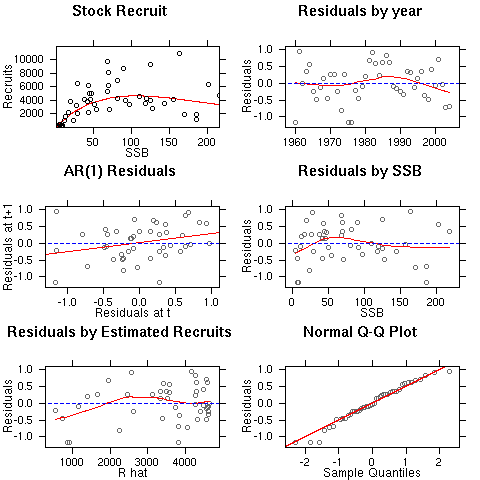
\includegraphics[width=1\textwidth]{FLSR_plot.png}
   \end{center}
\end{frame}

%A more complicated class with three levels: Fleet, Metier and Catch
%   \begin{center}
%      \includegraphics[width=1\textwidth]{/home/fas00/Work/Courses/Bergen/Presentation/fleet/FLFleet.png}
%   \end{center}
%********************************************
%\begin{frame}[plain]
%  \frametitle{FLEDA}
%@ 
%<<results=hide,echo=FALSE>>=
%library(FLEDA)
%ple4sex.spay <- spay(catch.n(ple4sex))
%# fine tune 
%ttl <- list(label="Standardized catch proportion at age for Plaice in IV", cex=1)
%yttl <- list(label="age", cex=0.8)
%xttl <- list(cex=0.8)
%ax <- list(cex=0.7)
%@
%%\end{frame}
%
%%\begin{frame}[plain]
%<<bubbles,echo=F,fig=T>>=
%# plot
%print(bubbles(age~year|unit, ple4sex.spay,  main=ttl, ylab=yttl, xlab=xttl, scales=ax, bub.scale=5))
%@ %def 
%\end{frame}
%
%************ Frame 15***********************
\begin{frame}
  \frametitle{Slot accessors}
      \begin{itemize}
	 \item<2-> Try to avoid using @ to access slots
	 \item<3-> Use accessors instead
	 \item<4-> e.g. landings.n(stock) not stock@landings.n
	 \item<5-> Protects against internal changes
	 \item<6-> e.g. catch slots removed from FLCatch
	 \item<7-> But accessor catch() still works
      \end{itemize}
\end{frame}
\end{document}

